\input{../../headers/beamercoursHeadings}

\section{Introduction}

{\frame{
\frametitle{Introduction}

\begin{savoir}
Vous êtes capables :
\begin{itemize}
 \item de résoudre des équations différentielles à l'aide des transformées de Laplace,
 \item de représenter des réponses impulsionnelles et indicielles,
 \item de représenter un SLCI à l'aide d'un schéma blocs. 
\end{itemize}
\end{savoir}

\begin{prob}
Vous devez êtes capables :
 \begin{itemize}
 \item d'effectuer l'étude harmonique d'un système,
 \item de représenter cette étude sur les diagrammes adéquats.
 \end{itemize}
\end{prob}
}}

{\frame{
\frametitle{Réponse harmonique}

Lorsque l'entrée d'un SLCI est un signal sinusoïdal du type $e(t)=E_0.sin(\omega_n.t)$, sa sortie en régime permanent est de la forme $s(t)=S_0.sin(\omega_n.t+f)$. 

\begin{center}
	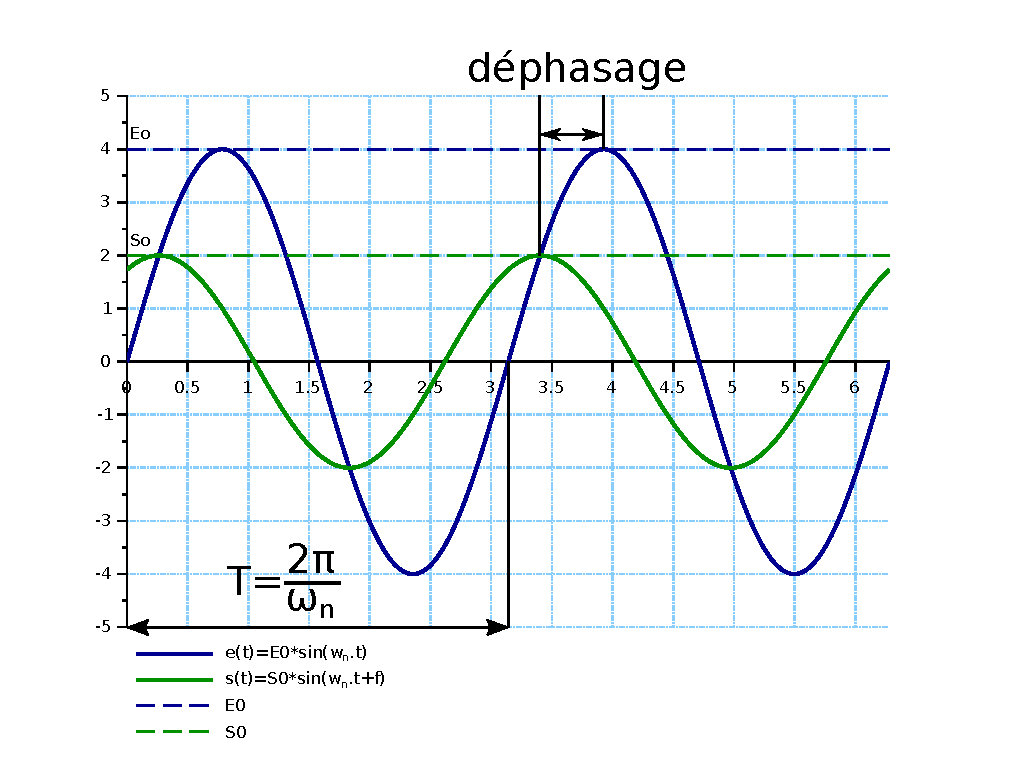
\includegraphics[width=0.5\linewidth]{img/harmo}
\end{center}

On appelle réponse harmonique, la sortie $s(t)$ en régime permanent d'un système soumis à une entrée $e(t)$ périodique. 
}}

{\frame{
\frametitle{Les diagrammes harmoniques}

Les courbes $e(t)$ et $s(t)$ dessinées ne sont valables que pour la pulsation $\omega_n$ du signal d'entrée. La représentation temporelle ne sera donc plus suffisante dans le cadre de cette étude.

\vfill

L'objet d'une étude fréquentielle d'un système est d'étudier l'évolution du \textbf{gain} et de la \textbf{phase}, en fonction de la variation de la valeur de la pulsation $\omega$ du signal d'entrée, sur la réponse harmonique du système.

\vfill

L'étude fréquentielle d'un système, consiste en l'étude, par la méthode des complexes, de la fonction de transfert du système H(p) : 
\begin{itemize}
 \item le \textbf{gain} du système $\frac{S_0}{E_0}$ qui est égal au module du nombre complexe $H(j\omega)$: $\frac{S_0}{E_0}=\vert H(j\omega) \vert$
 \item la \textbf{phase} du système $\varphi$ qui est égale à l'argument du nombre complexe $H(j\omega)$: $\varphi=arg(H(j\omega))$
\end{itemize}
}}


\section{Diagrammes de Bode}

{\frame{
\frametitle{Diagramme de Bode}

Plusieurs diagrammes permettent de décrire le comportement fréquentiel d'un système : Bode, Nyquist, Black. Dans un premier temps, nous nous limiterons à l'utilisation du diagramme de Bode.

Il est constitué de deux courbes correspondant aux tracés du module et la phase de $H(j\omega)$ en fonction de la pulsation sur une échelle logarithmique en base 10.

\vfill

\begin{minipage}{0.3\linewidth}
	\begin{itemize}
	 \item Le module $G_{db}=20\cdot log \vert H(j\omega) \vert$ est exprimé en décibel. 
	 \item La phase $\varphi$ est exprimée en degrés. 
	\end{itemize}
\end{minipage}
\hfill
\begin{minipage}{0.66\linewidth}
\centering
\def\svgwidth{0.75\columnwidth}
\input{img/bode1.pdf_tex}
\end{minipage}
}}

{\frame{
\frametitle{Cas du gain pur}

\begin{minipage}{0.48\linewidth}
\begin{center}
 \fbox{$H(p)=K$}
\end{center}
\end{minipage}
\hfill
\begin{minipage}{0.48\linewidth}
\begin{itemize}
 \item $G_{db}=20log\vert K \vert$  
 \item $\varphi=arg(K)=arctan\left(\dfrac{0}{K}\right)=0\textdegree$. 
\end{itemize}
\end{minipage}

\centering
\def\svgwidth{0.65\columnwidth}
\input{img/gain.pdf_tex}
}}

{\frame{
\frametitle{Cas de l'intégrateur}

\begin{minipage}{0.38\linewidth}
\begin{center}
 \fbox{$H(p)=\dfrac{K}{p}$}
\end{center}
\end{minipage}
\hfill
\begin{minipage}{0.58\linewidth}
\begin{itemize}
 \item $G_{db}=20log\bigg\vert \dfrac{K}{p} \bigg\vert=20log(K)-20log(\omega)$  
 \item $\varphi=arg\left(\dfrac{K}{j\omega}\right)=-arctan\left(\dfrac{\dfrac{\omega}{K}}{0}\right)=-90\textdegree$. 
\end{itemize}
\end{minipage}

\centering
\def\svgwidth{0.65\columnwidth}
\input{img/integrateur.pdf_tex}
}}

{\frame{
\frametitle{Cas du premier ordre}


\begin{minipage}{0.7\linewidth}
Pour $\omega \rightarrow 0$
\begin{itemize}
 \item $G_{db}=20log\bigg\vert \dfrac{K}{1+\tau.p} \bigg\vert=20log(K)-20log(1)=20log(K)$  
 \item $\varphi=arg\left(\dfrac{K}{1+\tau.j\omega}\right)=-arctan\left(\dfrac{0}{K}\right)=0\textdegree$.
 \end{itemize}
\end{minipage}\hfill
\begin{minipage}{0.27\linewidth}
\begin{center}
 \fbox{$H(p)=\dfrac{K}{1+\tau.p}$}
\end{center}
\end{minipage}
 
 Pour $\omega \rightarrow +\infty$
\begin{itemize}
 \item $G_{db}=20log\bigg\vert \dfrac{K}{1+\tau.p} \bigg\vert=20log\left(\dfrac{K}{\tau}\right)-20log(\omega)$  
 \item $\varphi=arg\left(\dfrac{K}{1+\tau.j\omega}\right)=-arctan\left(\dfrac{+ \infty}{K}\right)=-90\textdegree$. 
\end{itemize}

Pour $\omega=\omega_c=\dfrac{1}{\tau}$, pulsation de cassure.
\begin{itemize}
 \item $G_{db}=20log\left(\dfrac{K}{\sqrt{2}}\right)=20log(K)-3db$  
 \item $\varphi=arg\left(\dfrac{K}{1+\tau.j\omega_c}\right)=-arctan(1)=-45\textdegree$. 
\end{itemize}
}}

{\frame{
\frametitle{Cas du premier ordre}
\centering
\def\svgwidth{0.9\columnwidth}
\input{img/premier_ordre.pdf_tex}

}}

{\frame{
\frametitle{Cas du second ordre (z>1)}

\begin{center}
 \fbox{$H(p)=\dfrac{K}{1+\dfrac{2.z}{\omega_0}.p+\dfrac{p^2}{\omega_0^2}}$}
\end{center}

\textbf{Cas z>1}, alors $H(j\omega)=\dfrac{K}{(1+T_1.j.\omega).(1+T_2.j.\omega)}$

\vfill

\begin{itemize}
 \item $G_{db}=20log\bigg\vert \dfrac{K}{(1+T_1.j.\omega).(1+T_2.j.\omega)} \bigg\vert=20log(K)-10log(1+T_1^2.\omega^2))-10log(1+T_2^2.\omega^2))$  
 \item $\varphi=arg\left(\dfrac{K}{(1+T_1.j.\omega).(1+T_2.j.\omega)}\right)=-arctan\left(T_1.\omega\right)-arctan\left(T_2.\omega\right)$.
 \end{itemize}
 
Pour $\omega_0=\sqrt{\dfrac{1}{T_1.T_2}}$, la courbe de phase passe toujours par $-90\textdegree$.
}}

{\frame{
\frametitle{Cas du second ordre (z>1)}
\centering
\def\svgwidth{0.9\columnwidth}
\input{img/second_ordre_2.pdf_tex}

}}

{\frame{
\frametitle{Cas du second ordre (z=1)}

\begin{center}
 \fbox{$H(p)=\dfrac{K}{1+\dfrac{2.z}{\omega_0}.p+\dfrac{p^2}{\omega_0^2}}$}
\end{center}

\textbf{Cas z=1}, alors $H(j\omega)=\dfrac{K}{(1+T.j.\omega)^2}$

\vfill

\begin{itemize}
 \item $G_{db}=20log\bigg\vert \dfrac{K}{(1+T.j.\omega)^2} \bigg\vert=20log(K)-20log(1+T^2.\omega^2))$
 \item $\varphi=arg\left(\dfrac{K}{(1+T_1.j.\omega).(1+T_2.j.\omega)}\right)=-2.arctan\left(T.\omega\right)$.
 \end{itemize}
 
Pour $\omega_0=\sqrt{\dfrac{1}{T_1.T_2}}$, la courbe de phase passe toujours par $-90\textdegree$.
}}

{\frame{
\frametitle{Cas du second ordre (z=1)}
\centering
\def\svgwidth{0.9\columnwidth}
\input{img/second_ordre_1.pdf_tex}
}}


{\frame{
\frametitle{Cas du second ordre (z<1)}

\begin{center}
 \fbox{$H(p)=\dfrac{K}{1+\dfrac{2.z}{\omega_0}.p+\dfrac{p^2}{\omega_0^2}}$}
\end{center}

\textbf{Cas z<1}, alors $H(j\omega)=\dfrac{K}{1-\dfrac{\omega^2}{\omega_0^2}+j.\dfrac{2.z.\omega}{\omega_0}}$

\vfill

\begin{itemize}
 \item $G_{db}=20log\Bigg\vert \dfrac{K}{1-\dfrac{\omega^2}{\omega_0^2}+j.\dfrac{2.z.\omega}{\omega_0}} \Bigg\vert=20log(K)-10log\left(\left(1-\dfrac{\omega^2}{\omega_0^2}\right)^2+4.z^2.\left(\dfrac{\omega}{\omega_0}\right)^2\right)$
 \item $\varphi=arg\left(\dfrac{K}{1-\dfrac{\omega^2}{\omega_0^2}+j.\dfrac{2.z.\omega}{\omega_0}}\right)=
-arctan\left(\dfrac{\dfrac{2.z.\omega}{\omega_0}}{1-\dfrac{\omega^2}{\omega_0^2}}\right)$.
 \end{itemize}
}}

{\frame{
\frametitle{Cas du second ordre (z<1)}
\centering
\def\svgwidth{0.9\columnwidth}
\input{img/second_ordre.pdf_tex}
}}

{\frame{
\frametitle{Résonance}

Une résonance apparaît, lorsque $0<z<\dfrac{\sqrt{2}}{2}$, cela se manifeste par la présence d'un pic sur la courbe de gain.

Celui-ci étant un maximum, il peut être calculé s'il existe, pour la pulsation $\omega_r$ de la manière suivante: $\dfrac{dG}{d\omega}(\omega_r)=0$

\vfill

\begin{center}
$\left[\dfrac{d((\omega_0^2-\omega^2)^2+4.z^2\omega_0^2.\omega^2)}{d\omega}\right]_{\omega=\omega_r}=0$
\end{center}

\vfill

\begin{center}
$-4.\omega_r.(\omega_0^2-\omega_r^2)+8.z^2.\omega_0^2.\omega_r=0$.
\end{center}

\vfill

La résonance apparaît donc à la pulsation \fbox{$\omega_r=\omega_0.\sqrt{1-2.z^2}$}

\vfill

Et sa valeur est \fbox{$Q=\dfrac{|H(j.\omega)_{max}|}{|H(0)|}=\dfrac{1}{2.z.\sqrt{1-z^2}}$}.

}}

{\frame{
\frametitle{Conclusion}

\begin{savoir}
Vous êtes capables :
\begin{itemize}
 \item de construire les diagrammes de Bode à partir de fonctions de transfert,
 \item d'identifier des fonctions à partir de la lecture de ces diagrammes ou des tracés temporels.
\end{itemize}
\end{savoir}

\begin{prob}
Vous devez êtes capables :
 \begin{itemize}
 \item de mettre en place une correction de l'asservissement en vue du respect du cahier des charges.
 \end{itemize}
\end{prob}
}}


\end{document}